\section{Problemformulering}
Tracking af en lerdue i English Skeet \todo[inline, author=Anders]{eventuelt starte med en liste over forkortelser}(ES) vha. PTS. 
Lerduen er i vores opstilling udskiftet med en bold, men ellers følges reglerne for ES.
\todo[color=yellow! 100, inline, author=Anders]{Henvisning til litteraturliste eller fodnote}
Bolden bevæger sig i et 3D rum med negligerbar luftmodstand. \\

\begin{figure}[th!]
\centering
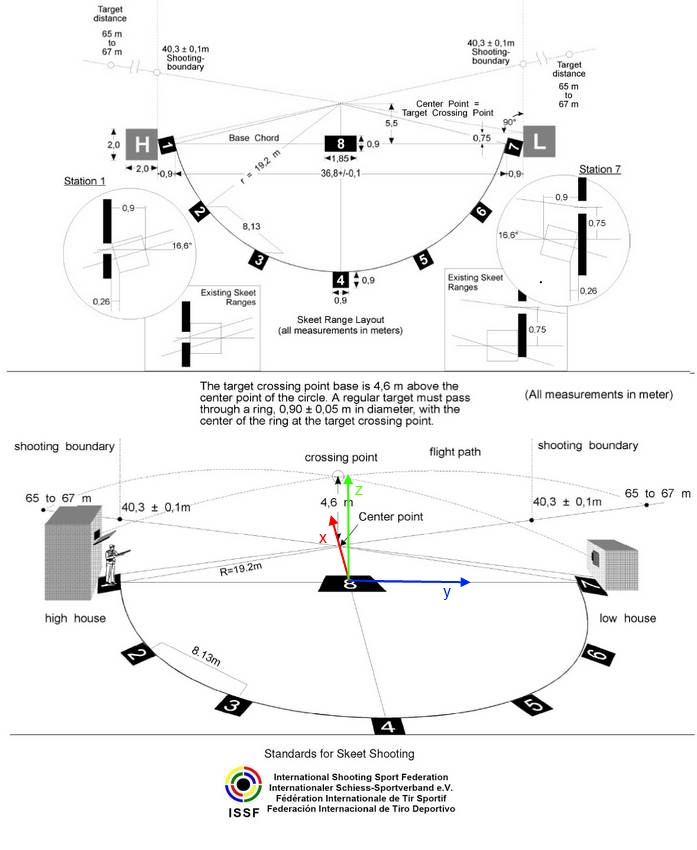
\includegraphics[width=0.4\textwidth]{./graphics/skeet-diagram_med_akser}
\caption[tekst i indholdsfortegnelsen]{figurtekst}
\label{fig:ES}
\end{figure}	
Systemets input er 60 kartesisiske koordinatsæt (x,y,z) per sekund. Hvor disse 
koordinater stammer fra, er uden for projektafgrænsningen. \\

Systemet dimensioneres til brug ifbm. en konkurrence i ES. En skitse over 
banen ses på figur \ref{fig:ES}. Det kartesiske koordinatsystem har origo i halvcirklens centrum, 
som indtegnet \todo[inline, author=Michael]{De er så indtegnet forkert.. Flot arbejde, klaphat..} 
nederst på figuren. I ES skal rammes serier af duer/mål der afskydes fra 
enten ”High House” eller ”Low House”, og med skud fra hver af de otte stationer langs 
cirkelperiferien. I dette projekt kigges kun på tilfældet hvor der afskydes mål fra ”High-
House” med pan-and-tilt systemet placeret på station 4.\\

Jævnfør reglerne for ES, skal duer/mål passere target crossing point (TCS) som er 
placeret i $4,57 [m]$ over origo. (0; 0; 4.57). Fejlmargin for passagen er $\pm0,45 [m]$. 
Målene skal desuden flyve $50 – 52 [m]$.  High house er placeret $20,11 [m]$ fra TCS, i en 
højde af $3,05 [m]$. Da luftmodstanden er negligerbar kan parablen (2. grads 
polynomium) findes ved at indsætte de kendte punkter. Herunder er parablen vist i et 
2D plan, figur \ref{fig:HH2D_para}.
\begin{figure}[!th]
\centering
\begin{tikzpicture}[scale=1]
\include*{./graphics/high_house_2D_parabola}
\end{tikzpicture}
\caption[Lerdue parabel]{Viser parablen af lerduens bane.}
\label{fig:HH2D_para}
\end{figure}
\todo[inline, author=Anders]{Den rigtige funktion skal sættes ind, afventer Michael}




Målet bliver affyret med en hastighed på $34 [m/s]$, i en vinkel på $9^{\circ}$ ift. xy-
planet. Set ovenfra bevæger målet sig som set på figur \ref{fig:para_in_xy_plane}. 
Figuren ses nedslagspunktet fra High-House, der er i alt $52 [m]$ startpositionen samt 
PTS placering i punktet B. 



\begin{figure}[!th]
\centering
\begin{tikzpicture}[scale=1]
\include*{./graphics/parabola_in_xy_plane}
\end{tikzpicture}
\caption[tekst i indholdsfortegnelsen]{figurtekst}
\label{fig:para_in_xy_plane}
\end{figure}

\todo[inline, author=Anders]{Jeg er gået igang med at tegne den og den kommer in snart.}

\subsection{Udregning af tallene}
\todo[inline, author=Michael]{Skal sikkert flyttes til appendix, hvis ikke det skal droppes helt? Bare så i kan se hvad jeg har haft gang i.}

For at simplificere udregningerne, regnes parablen kun i 2D. Det er trivielt at tilføje den tredje, så det gøres til sidst (hvis jeg finder det relevant). 

Kasteparablen er givet ved vektorfunktionen i ligning  \ref{eq:pf:vektorparabel}.

\begin{equation}
	Pos(t) = \left( \begin{array}{c}
	x(t) \\
	y(t)
	\end{array}
	\right)
	= \left( \begin{array}{c}
	\cos \theta v_0 t + x_0 \\
	\sin \theta v_0 t - \frac{g}{2} t^2 + y_0
	\end{array}
	\right)
\label{eq:pf:vektorparabel}
\end{equation}

Hvor $\theta$ er afskydningsvinklen, $v_0$ er afskydningshastigheden, $g$ er tyngdeacceleration og $x_0$,$y_0$ er begyndelsespunktet. 

For at få en parabel på formen y(x), isoleres t i x(t) med henblik på at substituere t i y(x): ($x_0$ sættes til 0.)

\begin{equation}
t = \frac{x}{\cos \theta v_0}
\label{eq:pf:x(t)}
\end{equation}

Den fundne værdi for t indsættes i $y(t)$, og udtrykket reduceres: 

\begin{eqnarray}
y(t(x)) &=& \sin \theta \frac{x}{\cos \theta v_0} v_0 - \frac{g}{2} \left(\frac{x}{\cos \theta v_0}\right)^2 + y_0 \\
y(x) &=& \tan \theta x - \frac{gx^2}{2(\cos \theta v_0)^2} + y_0
\label{eq:pf:y(x(t))}
\end{eqnarray}

Det ses at der er 3 ubekendte i ligningen. Dog er 3 punkter kendt fra HH parablen. Det er givet i reglerne for ESS at målet affyres fra en højde på 3.05 [m], så det indsættes i formlen. 
\begin{equation}
y(x) = \tan \theta x - \frac{gx^2}{2(\cos \theta v_0)^2} + 3.05
\label{eq:pf:y(x)2}
\end{equation}
Det er givet at målet skal passere TCS som er placeret i en højde på 4.57 [m], 20.11 [m] fra HH. 
Desuden skal målet bevæge sig 50 - 52 [m], i de videre beregninger 52 [m]. Det giver koordinatsættene (20.11; 4.57) og (52; 0). Vha. disse bestemmes $\theta$ og $v_0$ til:\footnote{Ved g = 9.82}
\todo[inline, author=Michael]{Måske giver det ikke mening med alle de decimaler, da det er udregnet med g = 9.82 - men jeg ved heller ikke hvor jeg skal finde en mere præcis måling af g?}
\begin{eqnarray}
\theta &=& 9.103 \degree \\
v_0 &=& 34.589 \frac{m}{s}
\end{eqnarray}
Disse parametre indsættes i vektorfunktionen fra ligning \ref{eq:pf:vektorparabel} samt udtrykket fra ligning \ref{eq:pf:y(x)2}. Udtrykkene reduceres: 
\begin{eqnarray}
	Pos(t) = \left( \begin{array}{c}
	x(t) \\
	y(t)
	\end{array}
	\right)
	&=& \left( \begin{array}{c}
	\cos \left(9.103 \degree \right) 34.589 t \\
	\sin \left(9.103 \degree \right) 34.589 t - \frac{9.82}{2} t^2 + 3.05
	\end{array}
	\right) \\
% ------------------------------
	&=& \left( \begin{array}{c}
	34.153 t \\
	- 4.91 t^2 5.473 t + 3.05
	\end{array}
	\right)
\label{eq:pf:vektorparabel2}
\end{eqnarray}

\begin{eqnarray}
y(x) &=& \tan \left(9.103 \degree \right) x - \frac{9.82x^2}{2(\cos \left(9.103 \degree \right) 34.589)^2} + 3.05 \\
% -------------------------------
&=& - 0.00421 x^2 + 0.1602 x  + 3.05
\label{eq:pf:y(x)3}
\end{eqnarray}